%%%%%%%%%%%%%%%%%%%%%%%%%%%%%%%%%%%%%%%%%%%%%%%%%%%%%%%%%%%%%%%%
\section{Particularités avec Python}
%%%%%%%%%%%%%%%%%%%%%%%%%%%%%%%%%%%%%%%%%%%%%%%%%%%%%%%%%%%%%%%%
\label{sec:particularites}

\begin{CadreAlgo}{\linewidth}{}
\textbf{Python} est un langage de programmation très utilisé dans le domaine scientifique. Il est complété par
différentes bibliothèques qui permettent de faire des calculs, de tracer des représentations graphiques
ou de générer des nombres aléatoires.
\end{CadreAlgo}

\medskip

\textbf{\large Exemples :}

$\star$ La bibliothèque \verb~math~ regroupe des fonctions mathématiques telles que racine carrée \verb~sqrt()~ et les
fonctions trigonométriques \verb~sin()~, \verb~cos()~, \verb~tan()~. 
Pour l'importer, on tape la commande :
\begin{lstlisting}
from math import *
\end{lstlisting}

$\star$ La bibliothèque \verb!random! regroupe des fonctions permettant de traiter des problèmes liés aux statistiques
et probabilités. 
Pour l'importer, on tape la commande :
\begin{lstlisting}
from random import *
\end{lstlisting}


$\star$ La bibliothèque \verb!pylab! regroupe les fonctions permettant le tracé de courbes représentatives de fonctions.
Pour l'importer, on tape la commande :
\begin{lstlisting}
from pylab import *
\end{lstlisting}


%\medskip

\begin{CadreAlgo}{\linewidth}{}
Les phrases précédées d'un dièse (\#) sont
des commentaires qui n'ont pas d'action sur le programme.

Elles peuvent être intéressantes pour expliquer ce qui est attendu du programme.
\end{CadreAlgo}

\medskip

\textbf{\large Exemple :}

\lstset{%
frame=single,% style du cadre - none pour ne pas encadrer
numbers=left,% numéros des lignes à gauche - none pour ne pas numéroter
numberstyle=\small,% on peut mettre \tiny ou \normalsize (taille par défaut)
firstnumber=0,% numéro de la première ligne
tabsize=6,% largeur des tabulations, 8 par défaut
showtabs=false,% permet de voir les tabulations quand true
xleftmargin=20pt,% marge gauche
xrightmargin=5pt,% marge droite qui peut rester à 0
framexleftmargin=0pt,% pour inclure les numéros dans le cadre : mettre 20pt
}

\begin{lstlisting}
from turtle import *
Screen() # Affiche une fenêtre
forward(100) # Trace un trait de 100 pixels vers la droite
circle(50,180) # Trace un 1/2 cercle de centre situe a 50 px a 
# gauche de la flèche (180 degrés pour faire un demi-tour)
\end{lstlisting}


%%%%%%%%%%%%%%%%%%%%%%%%%%%%%%%%%%%%%%%%%%%%%%%%%%%%%%%%%%%%%%%%
\section{Le tracé de figures avec le module turtle de Python}
%%%%%%%%%%%%%%%%%%%%%%%%%%%%%%%%%%%%%%%%%%%%%%%%%%%%%%%%%%%%%%%%


Dans l'exemple du \textbf{\ref{sec:particularites}}, on a déjà vu quelques instructions élémentaires du module \og turtle \fg{}.

Voici d'autres commandes qui peuvent être utiles :

\begin{lstlisting}
up() # Sous-entendu : pen up : pas de trace
forward(100) # Forward signifie : avance
right(90) # Tourne la tortue de 90 degrés vers sa droite
down() # Sous-entendu : pen down : on écrit !
back(100) # Recule de 100 pixels
\end{lstlisting}

\textbf{\large Exemple :}

\begin{lstlisting}
from turtle import *
shape("turtle") # Enfin une tortue qui ressemble a une tortue!
circle(50,180)
forward(100)
up()
forward(100)
right(90)
down()
back(100)
mainloop() # Permet de garder la fenêtre ouverte
\end{lstlisting}

Le programme ci-dessus donne la figure suivante :

\begin{center}
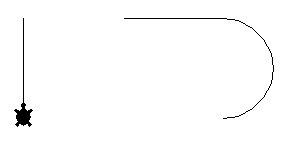
\includegraphics[width=0.5\textwidth]{turtle1}
\end{center}

Il existe bien d'autres commandes comme :

$\star$ \verb!left(nombre)! ou \verb!right(nombre)! : tourner la tortue de nombre degré vers sa gauche ou sa droite.

Exemple : \verb!left(180)! ou \verb!right(180)! font effectuer un demi-tour à la tortue.

$\star$ \verb!setx(nombre)! : définit l'abscisse de la tortue (son point de départ étant l'origine du repère $O(0\pv 0)$).

Exemple : \verb!setx(100)!

$\star$ \verb!sety(nombre)! : définit l'ordonnée de la tortue (son point de départ étant toujours l'origine $O(0\pv 0)$).

Exemple : \verb!sety(100)!

$\star$ \verb!goto(x,y)! : change la position de la tortue (x désigne l'abscisse, y l'ordonnée).

Exemple : \verb!goto(25,75)!

$\star$ \verb!setheading(nombre)! : définit l'orientation de la tortue. nombre représente un angle (en degrés
par défaut : 0 pour l'est, 90 pour le nord, 180 pour l'ouest, 270 pour le sud, etc.).

Exemple : \verb!setheading(30)!

$\star$ \verb!circle(rayon, angle)! : trace un cercle dans le sens contraire aux aiguilles d'une montre. Le
point de départ est situé à la position de la tortue, le centre est situé à un distance donnée
par rayon à gauche de la tortue. La portion du cercle tracée dépend de angle (mettre 360
— ou rien du tout! — pour un cercle complet). Si la valeur de rayon est négative, le cercle est
tracé dans le sens des aiguilles d'une montre, avec un centre situé à droite de la tortue!

$\star$ \verb!dot(taille, couleur)! : trace un disque dont le diamètre est gouverné par le paramètre optionnel
taille et la couleur définie par une chaîne de caractères désignant une couleur par son
nom (liste des noms de couleurs : \url{http://wiki.tcl.tk/37701}).

Exemple : \verb!dot(30, "pale green")! 

$\star$ \verb!stamp()! : dessine le symbole actuel de la tortue. Ce symbole peut être changé par la commande
\verb!shape(nom)!, où nom est une chaîne de caractères à choisir parmi "arrow", "turtle", "circle",
"square", "triangle" et "classic".

Exemple : \verb!shape("turtle") ; stamp()!

$\star$ \verb!width(taille)! : gouverne la largeur du trait (lorsque le crayon est abaissé).

Exemple : \verb!width(10)!

$\star$ \verb!color(couleur)! : définit la couleur du trait (les couleurs sont définies comme précédemment).

Exemple : \verb!color("DarkOrange1")!

$\star$ \verb!fillcolor(couleur)! : définit la couleur de remplissage.

Exemple : \verb!fillcolor("honeydew3")!

$\star$ \verb!bgcolor(couleur)! : définit la couleur du fond.

$\star$ \verb!begin_fill()! : à exécuter \textbf{avant} de tracer une forme dont on veut colorier l'intérieur.

Exemple : \verb!begin_fill() ; goto(75,25) ; stamp() ; goto(0,0) ; stamp() ;! 

\verb!forward(100) ; stamp() ; goto(25,75) ; stamp()!

$\star$ \verb!end_fill()! : à appeler \textbf{après} avoir tracé une forme dont on voulait colorier l'intérieur.

Exemple : \verb!end_fill()!

$\star$ \verb!mainloop()! : à appeler dans un script, pour empêcher la fenêtre de se fermer toute seule une
fois l'ensemble des tracés achevés.

Exemple : \verb!mainloop()!



%%%%%%%%%%%%%%%%%%%%%%%%%%%%%%%%%%%%%%%%%%%%%%%%%%%%%%%%%%%%%%%%
\section{L'affectation}
%%%%%%%%%%%%%%%%%%%%%%%%%%%%%%%%%%%%%%%%%%%%%%%%%%%%%%%%%%%%%%%%

Un programme informatique contient des instructions qui utilisent des variables prenant diverses valeurs
(valeurs numériques, booléens Vrai-Faux ou chaînes de caractères). Le langage Python (comme celui des calculatrices TI) ne requiert pas
de déclaration de variables.


L'affectation des variables se fait avec le symbole \og = \fg{}.

\textbf{\large Exemples :}

\verb!a = 2!  : \verb!a! prend la valeur 2.

\verb!b = 1.5! : \verb!b! prend la valeur 1,5. 

\danger Le séparateur décimal est un point et non pas une virgule.

\verb!c = 2%3! : \verb!c! prend la valeur égale au reste de la division euclidienne de 2 par 3.

\verb!d = 2/3! : \verb!d! prend la valeur du quotient décimal de 2 par 3.

\verb!e = 2*3! : \verb!e! prend la valeur du produit de 2 par 3.

\verb!f = 2**3! : \verb!f! prend la valeur de 2 puissance 3 (double signe * pour les puissances).

\verb!somme,n=0,100! : \verb!somme! prend la valeur 0 et \verb!n! la valeur 100.

%%%%%%%%%%%%%%%%%%%%%%%%%%%%%%%%%%%%%%%%%%%%%%%%%%%%%%%%%%%%%%%%
\section{Demander une valeur à l'utilisateur}
%%%%%%%%%%%%%%%%%%%%%%%%%%%%%%%%%%%%%%%%%%%%%%%%%%%%%%%%%%%%%%%%

La commande
\verb!a=int(input("Entrez le valeur de a : "))!
affiche le message entre guillemets et stocke la réponse de l'utilisateur (qui doit être un entier à cause de l'instruction \verb!int!) dans la variable \verb!a!.

En langage Python, on doit donc indiquer le type de variable attendu pour la réponse de l'utilisateur.

Voici des types de variables possibles :

$\star$ \verb!int! pour les entiers

$\star$ \verb!float! pour les nombres décimaux

$\star$ \verb!str! pour les chaînes de caractères


%%%%%%%%%%%%%%%%%%%%%%%%%%%%%%%%%%%%%%%%%%%%%%%%%%%%%%%%%%%%%%%%
\section{L'affichage}
%%%%%%%%%%%%%%%%%%%%%%%%%%%%%%%%%%%%%%%%%%%%%%%%%%%%%%%%%%%%%%%%

La commande \og print(\dots)\fg{} permet l'affichage du contenu entre parenthèses selon les règles décrites
ci-dessous :

\verb!print(a)! : Affiche la valeur de la variable a.

\verb!print('a')! :
Affiche la valeur de la lettre a (l'utilisation des guillemets
entraîne la copie du message entre guillemets).

\verb!print('a=',a)! : Affiche a= puis affiche la valeur de la variable a.

%%%%%%%%%%%%%%%%%%%%%%%%%%%%%%%%%%%%%%%%%%%%%%%%%%%%%%%%%%%%%%%%
\section{Effectuer des calculs}
%%%%%%%%%%%%%%%%%%%%%%%%%%%%%%%%%%%%%%%%%%%%%%%%%%%%%%%%%%%%%%%%


$\star$ 4 opérations classiques : $+ - * /$ Bibliothèque math

$\star$ $a$ exposant $b$ : \verb!a**b! 

$\star$ Racine carrée de $a$ : \verb!sqrt(a)!

$\star$ Division entière de $a$ par $b$ : \verb!a//b !

$\star$ Exponentielle de $a$ : \verb!exp(a)!

$\star$ Reste de la division euclidienne de $a$ par $b$ : \verb!a%b!

$\star$ Logarithme népérien de $a$ : \verb!log(a)!

et \verb!cos!, \verb!sin!, \verb!tan!\dots (angles en radians)

\medskip

\textbf{Nombres complexes}

$\star$ Définir $z$, nombre complexe : \verb!z=complex(3,2)!

En particulier, définir i : \verb!i=complex(0,1)!

$\star$ Valeur absolue, module de $z$ : \verb!abs(z)!

$\star$ Partie réelle, partie imaginaire de z :
\verb!z.real! et \verb!z.imag!

$\star$ Argument de $z$ (avec bibliothèque \verb!cmath!) :
\verb!phase(z)!

\medskip

\textbf{Bibliothèque} \verb!random!

$\star$ Nombre aléatoire dans $[0; 1[$ : \verb!random()!

$\star$ Nombre aléatoire entier entre $a$ et $b$ inclus :
\verb!randint(a,b)!





%%%%%%%%%%%%%%%%%%%%%%%%%%%%%%%%%%%%%%%%%%%%%%%%%%%%%%%%%%%%%%%%
\section{L'instruction conditionnelle}
%%%%%%%%%%%%%%%%%%%%%%%%%%%%%%%%%%%%%%%%%%%%%%%%%%%%%%%%%%%%%%%%

\begin{lstlisting}
if condition1 : # Ne pas oublier les deux points.
	instruction1 # Noter l indentation (espace)
elif condition2 : # Ce test est facultatif selon le problème
	instruction2
else : # Dernière condition.
	instruction
\end{lstlisting}


\textbf{\large Exemple :} Déterminer la plus petite de deux valeurs a et b entrées par l'utilisateur.

\begin{lstlisting}
def pluspetit(a,b):
    if a<b :
        return(a)
    else :
        return(b)
\end{lstlisting}

\begin{Rmq}[s]
$\star$ Les comparaisons possibles sont  :

\begin{center}
\begin{tabular}{c@{\hspace*{1em}:\hspace*{1em}}l}
== &égal à\\
!= &différent de\\
>  &strictement supérieur à \\
>= &supérieur ou égal à\\
<  &strictement inférieur à\\
<= &inférieur ou égal à
\end{tabular}
\end{center}

$\star$  Il est possible d'affiner une condition avec les mots clé \verb!AND! qui signifie \og ET\fg{} et \verb!OR! qui signifie \og OU\fg{}.

On veut par exemple tester si une valeur est plus grande que 5 mais aussi plus petite que 10 : 

\verb!if v>5 and v<10 :!

On peut également écrire \verb~if 5<v<10 :~
\end{Rmq}

\medskip

\begin{CadreAlgo}{\linewidth}{Simplification d'écriture}
On peut remplacer un test du type 
\verb~if x!=0:~
par \verb!if x:!.

Du coup, le test \verb!if x=0:! peut être remplacé par 
\verb!if not x:!
\end{CadreAlgo}

%%%%%%%%%%%%%%%%%%%%%%%%%%%%%%%%%%%%%%%%%%%%%%%%%%%%%%%%%%%%%%%%
\section{La boucle conditionnelle}
%%%%%%%%%%%%%%%%%%%%%%%%%%%%%%%%%%%%%%%%%%%%%%%%%%%%%%%%%%%%%%%%

On demande à l'utilisateur de choisir un nombre A (le seuil) et on cherche le premier entier $n$ tel que $2^n>A$ ($2^n$ dépasse le seuil).


\begin{lstlisting}
a=float(input("Quel est le seuil choisi ? "))
n=0
u=1
while u<a:
    n=n+1
    u=u*2
print("Seuil dépassé a partir de n=",n)
\end{lstlisting}




%%%%%%%%%%%%%%%%%%%%%%%%%%%%%%%%%%%%%%%%%%%%%%%%%%%%%%%%%%%%%%%%
\section{La boucle itérative}
%%%%%%%%%%%%%%%%%%%%%%%%%%%%%%%%%%%%%%%%%%%%%%%%%%%%%%%%%%%%%%%%

On cherche à calculer la somme des nombres de la forme $a^k$ pour $k$ allant de 0 à $n$, où $n$ est un entier naturel non nul choisi par l'utilisateur.

\begin{lstlisting}
print("Nous allons calculer la somme des a^k")
a=int(input("Quel est l'entier a choisi ? "))
n=int(input("Quel est l'entier n choisi ? "))
S=0
for k in range(n+1):
    S=S+a**k
print("La somme est ",S)
\end{lstlisting}

\begin{Rmq}[s]
$\star$ Python propose une instruction \og \verb!for! \textit{variable} \verb!in! \textit{liste} :\fg{} qui permet d'exécuter un bloc d'instructions (dont l'ouverture est signalée par le symbole :) en donnant successivement à la variable les différentes valeurs de la liste.

$\star$ Pour retrouver le comportement du bloc répéter 6 fois de Scratch, il suffira d'utiliser l'instruction \og \verb!for i in range(6):!\fg{} puisque \verb!range(6)! permet d'itérer sur la liste \verb![0,1,2,3,4,5]!. 

$\star$ Plus généralement \verb!range(a,b)! permet d'itérer sur la liste des entiers compris entre \verb!a! (inclus) et \verb!b! (exclu).
\end{Rmq}

\begin{Exemple}[]{}
Le programme suivant permet de calculer la moyenne des 100 premiers nombres entiers impairs :
\end{Exemple}

\begin{lstlisting}
somme,n = 0,100
for x in range(n):
	somme = somme + 2*x+1
	moyenne = somme/n
\end{lstlisting}



%%%%%%%%%%%%%%%%%%%%%%%%%%%%%%%%%%%%%%%%%%%%%%%%%%%%%%%%%%%%%%%%
\section{Les fonctions algorithmiques}
%%%%%%%%%%%%%%%%%%%%%%%%%%%%%%%%%%%%%%%%%%%%%%%%%%%%%%%%%%%%%%%%
\subsection{Utilisation simple}
%%%%%%%%%%%%%%%%%%%%%%%%%%%%%%%%%%%%%%%%%%%%%%%%%%%%%%%%%%%%%%%%

Le langage Python utilise fréquemment des \textbf{fonctions} pour effectuer les traitements attendus.

Une \textbf{fonction} est un programme qui utilise un ou plusieurs paramètres de différents types (numérique,
booléen ou chaîne de caractères).

Elle est définie par son nom et ses paramètres : \verb!fonction(paramètre1,paramètre2...)!.

Lorsqu'une fonction est appelée, elle renvoie un résultat numérique, un booléen ou une chaîne de caractères,
c'est-à-dire que l'utilisateur lit sur l'écran un résultat.

La syntaxe d'une fonction est du type :

\begin{lstlisting}
def fonction(paramètres) :
	instructions
	return(...)
\end{lstlisting}

Ces fonctions peuvent renvoyer un message, une(des) valeur(s) numérique(s) ou un booléen (Vrai ou
Faux), comme dans l'exemple ci-dessous.

\begin{lstlisting}
def affine(a) : # Ne pas oublier les deux points.
	y = 3*a-5 # Calcul.
	return(y) # Affichage du résultat.

\end{lstlisting}

Pour calculer l'image de 2 par la fonction \verb!affine()! définie ci-dessus, on appelle cette fonction en tapant
la commande : \verb!affine(2)!. On obtient l'affichage : 1.

\medskip

\begin{Rmq}[]
Une \textbf{procédure} est définie comme une \textbf{fonction},
mais elle ne comprend pas l'instruction return.
\end{Rmq}

%%%%%%%%%%%%%%%%%%%%%%%%%%%%%%%%%%%%%%%%%%%%%%%%%%%%%%%%%%%%%%%%
\subsection{Utilisation plus évoluée}
%%%%%%%%%%%%%%%%%%%%%%%%%%%%%%%%%%%%%%%%%%%%%%%%%%%%%%%%%%%%%%%%
\subsubsection{Fonction récursive}
%%%%%%%%%%%%%%%%%%%%%%%%%%%%%%%%%%%%%%%%%%%%%%%%%%%%%%%%%%%%%%%%

Une fonction \textbf{récursive} est une fonction qui s'appelle elle-même.

L'usage de fonctions récursives fournit un code élégant, mais qui demande un certain effort intellectuel
pour comprendre son fonctionnement. 

De plus, il faut être attentif aux conditions utilisées : encore plus
qu'avec un while, le danger d'une boucle infinie est présent.

\medskip

\textbf{\large Exemple :} pgcd de deux entiers avec une fonction récursive

À comparer avec le pgcd classique fondé sur une boucle while.

\begin{lstlisting}
def pgcd_recursif(a,b):
	r = a%b # Reste dans la division euclidienne de a par b
	if r==0 :
		# Si le reste est nul : on renvoie b
		return b
	else :# Sinon : on calcule le pgcd de b et r
		return pgcd_recursif(b,r)
\end{lstlisting}

%%%%%%%%%%%%%%%%%%%%%%%%%%%%%%%%%%%%%%%%%%%%%%%%%%%%%%%%%%%%%%%%
\subsubsection{Appliquer une fonction sur chaque item d'un élément itérable}
%%%%%%%%%%%%%%%%%%%%%%%%%%%%%%%%%%%%%%%%%%%%%%%%%%%%%%%%%%%%%%%%

On utilise une instruction du type \verb!map(function,[])!

\begin{lstlisting}
>>> def add_one(x): return x + 1
>>> list(map(add_one, [1,2,3]))
[2, 3, 4]
\end{lstlisting}


%%%%%%%%%%%%%%%%%%%%%%%%%%%%%%%%%%%%%%%%%%%%%%%%%%%%%%%%%%%%%%%%
%\newpage
\section{Simulation du hasard}
%%%%%%%%%%%%%%%%%%%%%%%%%%%%%%%%%%%%%%%%%%%%%%%%%%%%%%%%%%%%%%%%

On cherche à simuler le lancer cubique à 6 faces dont les faces sont numérotées de 1 à 6 un nombre de fois N choisi par l'utilisateur et à calculer la fréquence d'apparition de la face 6 dans cette série.

Pour simuler le choix au hasard d'un entier, on utilise la fonction \verb!randint! de la bibliothèque \verb!random!.

\begin{lstlisting}
from random import *
n=int(input("Combien de lancers souhaitez vous ? "))
S=0
for k in range(n):
    a=randint(1,6)# on tire au hasard un nombre entier 
    #parmi 1,2,3,4,5,6
    if a==6:
        S=S+1
print("La fréquence des 6 sur cet échantillon")
print("de ",n," lancers est ",S/n)
\end{lstlisting}

La fonction \verb!choice([])! de la bibliothèque \verb!random! retourne une valeur d'une liste aléatoirement. 

\begin{lstlisting}
>>> import random
>>> random.choice([1,2,3,4,5])
3
>>> random.choice([1,2,3,4,5])
2
>>> random.choice(['x','abcde','hello','yes!'])
'yes!'
\end{lstlisting}

%%%%%%%%%%%%%%%%%%%%%%%%%%%%%%%%%%%%%%%%%%%%%%%%%%%%%%%%%%%%%%%%
\section{L'utilisation des chaînes de caractères}
%%%%%%%%%%%%%%%%%%%%%%%%%%%%%%%%%%%%%%%%%%%%%%%%%%%%%%%%%%%%%%%%

$\star$ Concaténer deux chaînes \og abc\fg{} et \og def\fg{} : \verb~"abc"+"def"~

$\star$ Obtenir le caractère numéro \verb~i~ de la chaîne \verb~chaine~ : \verb~chaine[i]~

Cela fonctionne comme pour une liste.

$\star$ Convertir la chaîne de caractères \og 123\fg{} en un entier : \verb~int("123")~

$\star$ Convertir l'entier \og 123 \fg{}  en chaîne de caractères : \verb~str(123)~

$\star$ Convertir la liste \verb~List~ en chaîne de caractères, les éléments étant séparés par \og - \fg{}, puis stocker le résultat dans la chaîne \verb~chaine~ : \verb~chaine="-".join(List)~

%%%%%%%%%%%%%%%%%%%%%%%%%%%%%%%%%%%%%%%%%%%%%%%%%%%%%%%%%%%%%%%%
\section{L'utilisation de listes}
%%%%%%%%%%%%%%%%%%%%%%%%%%%%%%%%%%%%%%%%%%%%%%%%%%%%%%%%%%%%%%%%


$\star$ Initialiser une liste L vide : \verb!L = []!

$\star$ Initialiser une liste L contenant 6 termes égaux à 0 : \verb!L = 6*[0]!

$\star$ Affiche la valeur d'indice $i$ de la liste L (le premier indice est 0) :
\verb!L[i]!

$\star$ Affecter la valeur $a$ à la valeur d'indice $i$ de la liste L (le premier indice est 0) :
\verb!L[i]=a!

$\star$ Ajouter l'élément x au bout de la liste L :
\verb!L.append(x)! ou \verb~L=L+[x]~ ou \verb~L+=[x]~

$\star$ Ajouter l'élément x au rang i de la liste L :
\verb!L.insert(i,x)!

$\star$ Supprimer la première occurrence de x dans la
liste L : \verb!L.remove(x)!

$\star$ Supprimer l'élément d'indice $i$ dans la liste L :
\verb!L.pop(i)! ou \verb!del L[i]!

\verb~L.pop()~ supprime le \textbf{dernier} élément de la liste L

$\star$ Longueur d'une liste L :
\verb!len(L)!

$\star$ Trier une liste L et stocker le résultat dans
\verb!L_triee! :
\verb!L_triee = sorted(L)!

$\star$ Inverser l'ordre des éléments de la liste L :
\verb!L.reverse()! ou  \verb~L[::-1]~

\danger Il y a une différence notable entre les deux solutions :

\verb!L.reverse()! modifie la liste L (ainsi que les autres listes qui lui sont égales), alors que
\verb~M=L[::-1]~ ne modifie pas la liste L.

Au lieu de \verb!M=L[::-1]!, on peut également utiliser 
\verb!M=L[:]! ou \verb!M=L.copy()!

$\star$ Compter le nombre d'occurrences de $a$ dans la liste L :
\verb!L.count(a)!

$\star$ \verb!L[::3]! renvoie une liste formée des termes de L de rang multiple de 3.

$\star$ \verb!L[::2]! renvoie une liste formée des termes de L de rang multiple de 2.

\medskip

\textbf{\large Exemple}

\begin{lstlisting}
def syracuse(n):
    L = [n]
    while (n!=1):
        if (n%2==0): # Test de parité
            n = (n//2) # Division entière
        else:
            n = n*3+1
        L.append(n)
    return L

import matplotlib.pyplot as plt

def graph_syracuse(nombre):
    Y_liste = syracuse(nombre) # On remplit la liste Y_liste
    # avec les valeurs de la suite de Syracuse
    X_liste = [] # Initialisation de la liste des abscisses
    for i in range(1,len(Y_liste)+1): # Affectation des 
    #indices de la suite
        X_liste.append(i)
    plt.plot(X_liste,Y_liste,"b.") # Création du graphique et 
    #affichage
\end{lstlisting}

%%%%%%%%%%%%%%%%%%%%%%%%%%%%%%%%%%%%%%%%%%%%%%%%%%%%%%%%%%%%%%%%
\section{Les graphiques de fonctions mathématiques}
%%%%%%%%%%%%%%%%%%%%%%%%%%%%%%%%%%%%%%%%%%%%%%%%%%%%%%%%%%%%%%%%

La bibliothèque \verb!matplotlib! et son module \verb!pyplot! sont conçus de manière à tracer des graphiques point
par point de façon rapide\dots à condition de se plier à leur pratique.

Soit à tracer la parabole d'équation $y=x^2$ sur l'intervalle $\intervalleff{-2}{2}$, avec un pas de 0.001 : quatre milliers de
points suffisent à faire une étude comparative de vitesse de tracé, à l'aide de la bibliothèque \verb!time!.

Pour pouvoir tracer des courbes de fonctions mathématiques nous allons donc charger le module \verb!pyplot! de la bibliothèque \verb!matplotlib!.

Comme c'est un peu long, on peut modifier le nom avec l'instruction 

\verb!import matplotlib.pyplot as plt!.


L'instruction \verb!plot! de \verb!matplotlib.pyplot! est optimisée pour tracer des graphiques utilisant des listes. 

Il faut raisonner en termes de \og tableau de valeurs \fg{} :

$\star$ X et Y sont deux listes de même longueur : par exemple $[1,2,3]$ et $[1,4,9]$.

$\star$ \verb!plt.plot(X,Y,".b")! trace l'ensemble des points $(X[i] ,Y[i])$ : (1,1), (2,4) et (3,9).

L'essentiel du programme consiste donc à alimenter les deux listes X et Y, à l'aide de la commande \verb!append!.

\begin{lstlisting}
import matplotlib.pyplot as plt

def courbe(f,a,b):
    X = []
    Y = []
    for k in range(a,b+1) :
        X.append(k)
        Y.append(f(k))
    plt.plot(X,Y,"b-")#trace la courbe en bleu, les points 
    #etant relies
    plt.show()


def courbe_pas(f,a,b,pas):
    X = []
    Y = []
    while a <= b :
        X.append(a)
        Y.append(f(a))
        a = a + pas
    plt.plot(X,Y,"g-")#trace la courbe en vert, les points 
    #etant relies
    plt.show()


import time #pour calculer le temps d'exécution du programme
def trace_courbe_fct(f,a,b,pas):
    depart=time.perf_counter()
    X = [] # Initialisation des listes
    Y = []
    while a<=b:
        X.append(a) # Ajout des valeurs
        Y.append(f(a)) # au "bout" de X et Y
        a = a+pas
    # Trace de l'ensemble du tableau de valeurs
    plt.plot(X,Y,"r.")#trace la courbe en rouge, les points 
    #n'etant pas relies
    plt.show()
    fin=time.perf_counter()
    return "Temps : " + str(fin-depart) + " s."
\end{lstlisting}

\textbf{\large Quelques instructions}

$\star$ Placer un point de coordonnées $(x; y)$, en bleu, gros :
\verb!plt.plot(x,y,"bo")!

$\star$ Tracer un segment entre deux points A et B, rouge :
\verb!plt.plot([xA,xB],[yA,yB],"r")!

$\star$ Tracer les points dont les coordonnées sont données par les listes \verb!X_liste! et \verb!Y_liste!, en noir, en reliant les points :
\verb!plt.plot(X_liste,Y_liste,"k-")!

$\star$ Pour avoir un repère orthonormé :
\verb!plt.axis("equal")!

$\star$ Pour une grille :
\verb!plt.grid()!

$\star$ Afficher la fenêtre graphique :
\verb!plt.show()!

\medskip

\textbf{\large Couleurs et style}

\begin{center}
\begin{tabular}{c@{\hspace*{1em}:\hspace*{1em}}l|c@{\hspace*{1em}:\hspace*{1em}}l}
b& bleu& - &ligne continue\\
g& vert& – &tirets\\
r& rouge& : &pointillés\\
c& cyan& . &points\\
m& magenta& o &billes\\
y& jaune& x &croix\\
k &noir& v &triangles\\
w &blanc &-. &point-tirets
\end{tabular}
\end{center}